\documentclass{article}
\usepackage[margin=1in]{geometry}
\usepackage{graphicx}
\usepackage{hyperref}
\usepackage{natbib}
\usepackage{soul}
\bibliographystyle{apalike}
\usepackage{amsmath}

\title{Fish can fly}

\author{Aden Ip$^1$\textbf{*} \and
Gledis Guri$^1$\textbf{*} \and
Elizabeth Andruszkiewicz Allan$^1$ \and
Ryan P. Kelly$^1$}

\date{\today}

\begin{document}

\maketitle

\section*{}

\begin{center}
\begin{tabular}{ll}
1 & School of Marine and Environmental Affairs, University of Washington, Seattle, Washington, USA \\
\hline
\textbf{*} & shared first authorship\\
&\\
& corresponding author \textbf{adenip@uw.edu}
\end{tabular}
\end{center}

\section*{Teaser}
Aquatic life leaves traces in the air, unveiling a new frontier in passive biodiversity monitoring.

\section*{Abstract}
Aquatic life can now be detected and quantified from the air. We demonstrate, for the first time, that airborne environmental DNA (eDNA)—genetic material transported from water into the atmosphere via natural processes like evaporation, aerosolization, and splashing—can be passively collected and used to track aquatic species abundance with high fidelity. This novel framework offers a safer, simpler, and more scalable alternative to conventional survey methods. Traditional techniques like netting, trapping, and visual surveys are logistically demanding and geographically constrained, while water-based eDNA sampling, though non-invasive, still relies on pumps, cold storage, and complex field logistics. Airborne eDNA bypasses these challenges, offering a tool that requires no water access and minimal equipment. We tested four passive airborne eDNA collection methods in salmon spawning streams: three air filters (gelatin, PTFE, MCE) and an open container of deionized water. These were benchmarked against water-based eDNA samples and direct visual fish counts. Quantitative PCR assays and Bayesian hierarchical modeling revealed strong correlations between airborne DNA concentrations and observed salmon density. The open DI water container achieved the highest overall recovery, PTFE filters delivered the most reproducible results, and gelatin filters showed the greatest sensitivity but higher environmental variability. This is the first study to link airborne eDNA to real-time aquatic population trends with statistical rigor. Our findings expand the spatial domain of aquatic monitoring into the atmosphere, highlight the ecological connectedness between air and water, and provide a foundation for low-impact, high-resolution biodiversity surveillance. This framework opens new frontiers for environmental genomics, conservation biology, ecosystem and public health management in a rapidly changing world.\\

\textbf{Keywords}: environmental DNA, Air eDNA, Passive Air Filtration, Aquatic Biomonitoring, Aerosolization, Evaporation, Non-invasive Sampling, Quantitative eDNA Analysis, Salmon, Environmental Genomics

\section{Introduction}
Monitoring aquatic life is fundamental for understanding ecosystem health, guiding conservation efforts, and managing invaluable natural resources. Traditional fish surveys, including direct visual counts, netting, and trapping, have long served as the backbone of aquatic monitoring. However, these methods are labor-intensive, expensive, and logistically challenging (REF; Guri et al., 2024b???). Such constraints often restrict sampling to easily accessible locations and may cause critical ecological dynamics in remote or hazardous environments to be overlooked (REF). This has created demand for alternative approaches that reduce logistical burden while expanding spatial and temporal reach. In addition, the extensive manpower and specialized equipment required further limit the frequency and geographic scale of routine monitoring (REF).  

Recent advances in environmental DNA (eDNA) techniques have revolutionized biodiversity assessment by detecting organisms through the genetic material they shed into their surroundings (REF). Water-based eDNA assays have repeatedly proven effective for confirming species presence, offering a non-invasive alternative to traditional surveys (REF). Yet, these methods typically require complex field operations and cumbersome logistics, including the transport of heavy equipment and meticulous handling of water samples, which hinder continuous or large-scale implementation (REF). In some cases, direct access to water bodies is physically dangerous or impossible, such as in steep waterfalls or stagnant waters where microbial hazards may pose risks to human health (REF. Additionally, while water-based eDNA reliably detects species presence, it frequently falls short of capturing dynamic ecological processes or providing robust, quantitative links between DNA concentration and actual organism abundance (REF).

 These limitations not only challenge the sufficiency of water-based monitoring alone but also invite a broader rethinking of where and how ecological signals are collected. Environmental systems are inherently interconnected, and biological material is not confined to a single medium. This opens new frontiers for biomonitoring beyond aquatic habitats. One such frontier is airborne eDNA: genetic material that is aerosolized or splashed from aquatic systems into the atmosphere, where it may be carried, diluted, and redeposited. If detectable, these airborne signals could offer a low-impact, scalable extension of aquatic biomonitoring into the air—potentially yielding presence and abundance information without needing direct contact with water.

Building on these technological advances, the current study introduces airborne eDNA sampling as a transformative approach to aquatic biomonitoring. This framework is based on the hypothesis that natural processes such as evaporation, aerosolization, and splashing transfer DNA molecules from aquatic habitats into the overlying air, effectively turning the atmosphere into a diluted yet informative extension of the water column (Figure \ref{fig:AI_physical_model}). Salmon, a keystone species known not only for their critical role in nutrient cycling and energy transfer but also for their vigorous spawning behavior that includes leaping and jumping, serve as an ideal test case. Their dynamic activity is expected to enhance the dispersal of DNA molecules from water into the air, providing an effective model for evaluating airborne eDNA collection. To rigorously evaluate this concept, four distinct collection methods were compared: passive air filters constructed from gelatin (commonly used in low-flow air filtration systems), PTFE (standard in high-flow air applications), and MCE (traditionally employed for water filtration), as well as an open container of deionized water exposed to ambient conditions (REF). This comprehensive comparison enables the assessment of both the detection sensitivity and the quantitative capacity of each method to reflect aquatic life dynamics.

Despite the promise of eDNA approaches, fundamental limitations persist in how aquatic biodiversity is monitored. Water-based eDNA methods, while effective, depend on logistically intensive protocols that restrict their use in remote, hazardous, or resource-limited settings (REF). These limitations have sparked interest in airborne eDNA as a novel frontier in aquatic monitoring. Airborne eDNA has recently emerged as a conceptually promising extension—one that could eliminate the need for pumps, water access, or complex sampling gear, and allow for simpler, passive, and scalable monitoring strategies (REF). However, this potential remains unrealized. To our knowledge, this is the first study to demonstrate that airborne eDNA can reliably detect aquatic organisms. We also establish, for the first time, a quantitative link between airborne DNA concentrations and underlying aquatic species abundance using statistical modeling. Together, these findings represent a conceptual leap, showing that aquatic life can be tracked through the air and that these signals quantitatively reflect real-world population trends. This opens the door to robust, real-time ecological inference from the atmosphere. In the absence of validated methods and models, the utility of airborne eDNA for aquatic systems has remained speculative. Addressing this gap is essential to develop a truly low-impact, scalable, and continuous monitoring framework capable of operating where conventional techniques fall short.

The primary objective of this study is not merely to validate passive airborne sampling, but to introduce a novel framework for capturing aquatic eDNA from the air. By drawing on principles from airborne particulate filtration and repurposing materials commonly used in air microbiology, we systematically evaluated whether environmental DNA from aquatic systems can be collected passively through gravitational settling. We proposed and tested a set of complementary sampling materials, PTFE, gelatin, MCE filters, and an open container of water as a particle settlement collector; chosen for their distinct physical properties and hypothesized affinities for settling DNA particles. By integrating these designs with the “air is dilute water” hypothesis, we demonstrate a conceptual and technical advance in how aquatic eDNA can be detected. The resulting approach offers substantial advantages in safety, scalability, and cost-efficiency, opening a new frontier for non-invasive, real-time biomonitoring. Although the study focuses on salmon, the broader potential of this framework extends to a wide range of aquatic organisms. The findings not only simplify field operations by reducing logistical demands and operational risks but also reveal that ecological signals are not confined to water bodies. Rather, the air can serve as an additional, quantifiable reservoir of biodiversity data. Collectively, these results lay the groundwork for transforming ecological monitoring into a more comprehensive, real-time process capable of improving resource management in rapidly changing environments.

\begin{figure}[tbhp] 
\centering
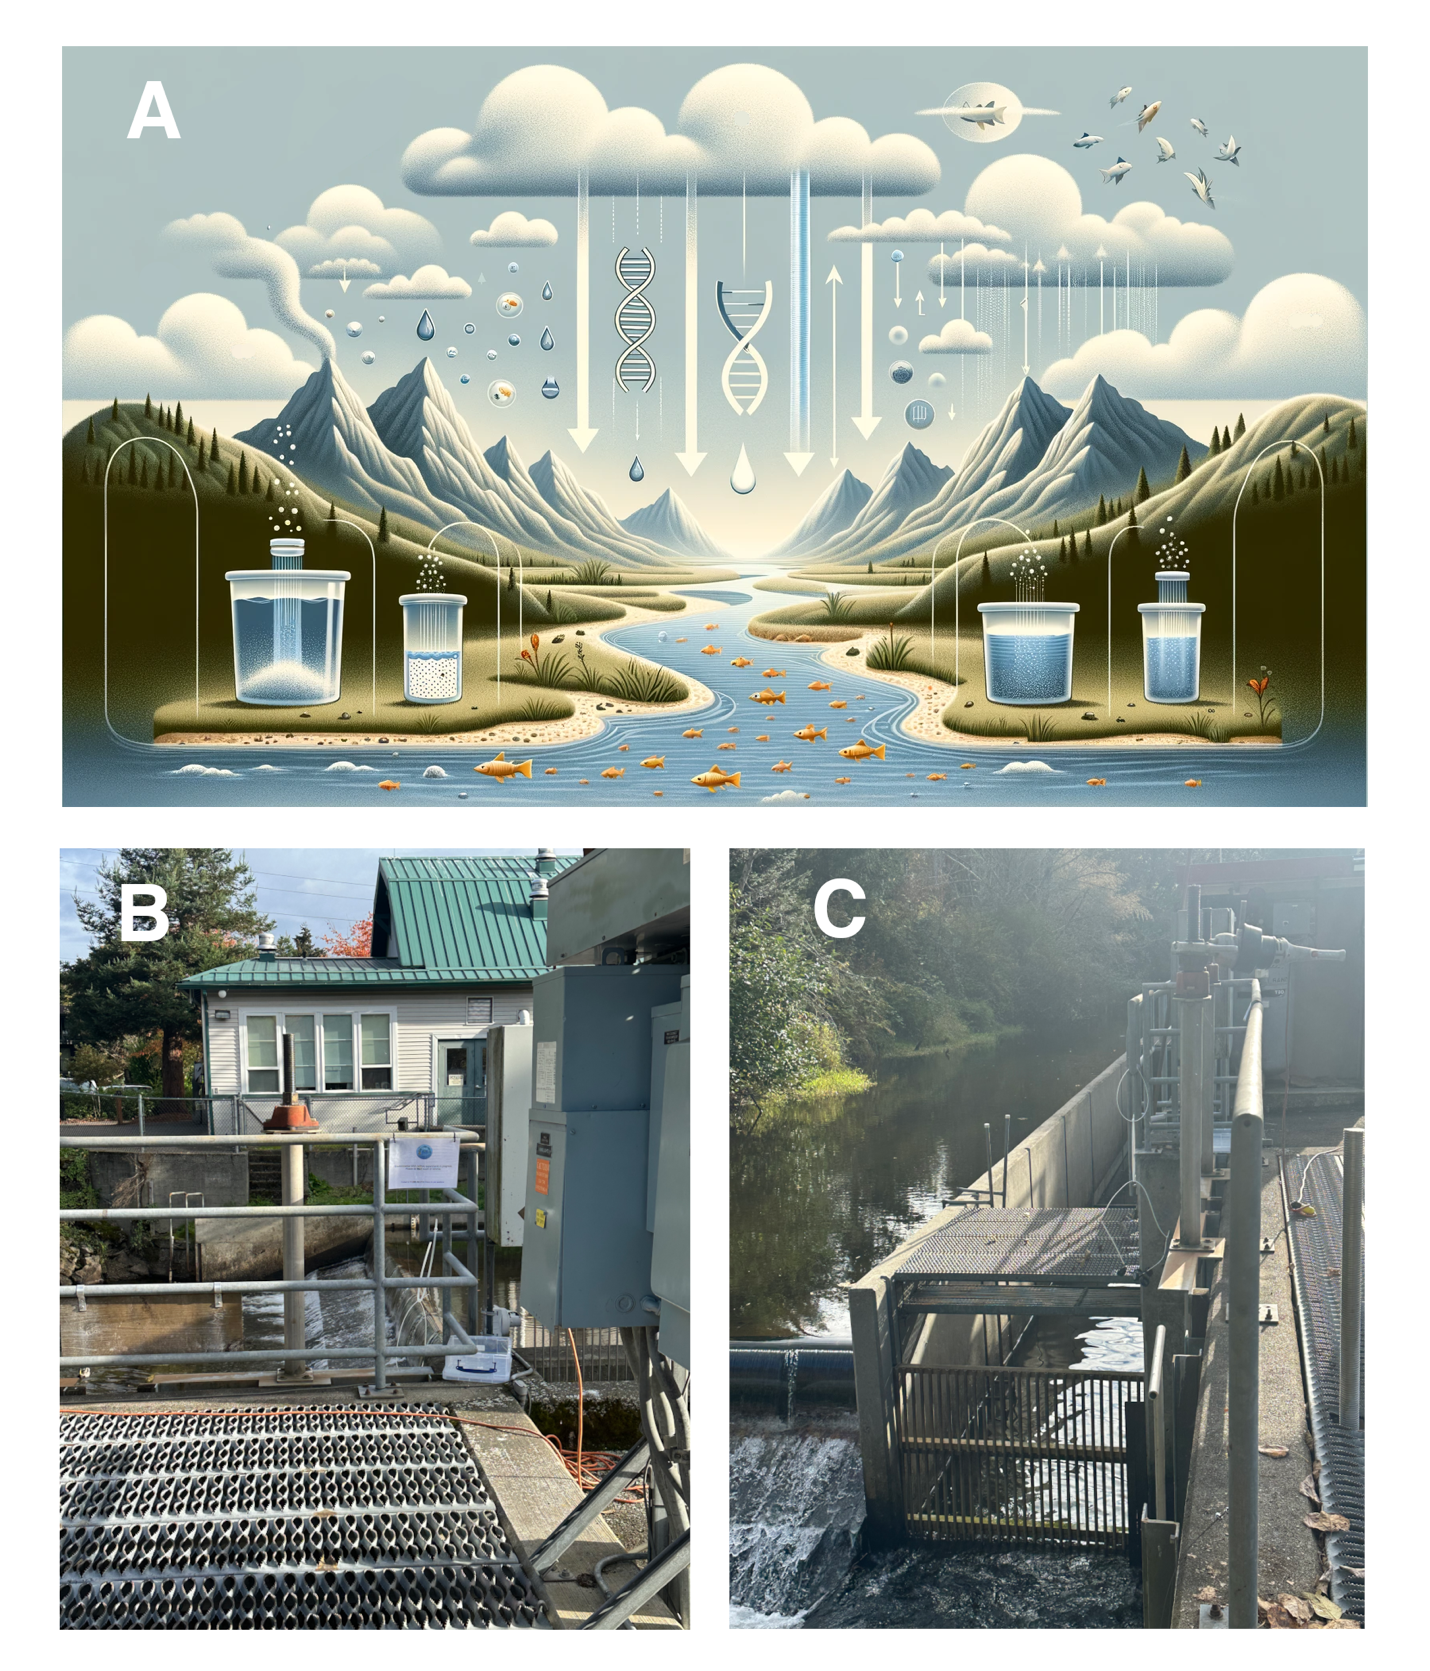
\includegraphics[width=13.5cm]{Plots/Picture1.png}  
\caption{(A) Conceptual illustration of how aquatic environmental DNA (eDNA) is transported from water into the atmosphere and subsequently captured by passive sampling devices. Natural processes, including evaporation, aerosolization, and splashing, transfer trace amounts of eDNA from a river ecosystem into the air, where four passive airborne particle collectors recover the DNA molecules as it settles. Arrows highlight the movement of DNA-containing droplets from water to air and into sampling devices, suggesting the possibility of collecting airborne eDNA detection for aquatic biomonitoring. (B) Field deployment of the open container and air filters along a hatchery railing. The tray of water is visible at the lower right. (C) The air filters (PTFE, gelatin, and MCE) are hung approximately 30 cm below, and are positioned beside the open water container, about 3 m above the water’s surface. This configuration minimizes splash contamination and captures airborne DNA particles driven by gravitational settling. The positioning relative to flowing water demonstrates how these passive collectors operate at a vantage point above the stream, facilitating non-invasive DNA capture in real-world field conditions.}
\label{fig:AI_physical_model}
\end{figure}

\section{Methods}

\subsection{Field Sampling}

The study was conducted in salmon spawning streams outside of the Issaquah Salmon Hatchery (47.529501$^\circ$ N, 122.039133$^\circ$ W) from 26 August 2024 to 18 November 2024, with nine sampling trips. Given our focus on coho salmon (Oncorhynchus kisutch) and our knowledge of their spawning window—with peak abundance observed from 17 October 2024 onward—sampling was strategically timed to capture the lowest to highest levels of eDNA release. Visual counts were performed by hatchery staff, and salmon escapement data were obtained from the Washington Department of Fish and Wildlife escapement reports (\href{https://wdfw.wa.gov/fishing/management/hatcheries/escapement#2024-weekly}{https://wdfw.wa.gov/fishing/management/hatcheries/escapement\#2024-weekly}). Environmental conditions varied across sampling events, ranging from fair weather to heavy rain (see Supplementary Material 1 for detailed meteorological records).

Sampling was conducted in 24-hour blocks. On the first day, filters and an open container of deionized water were deployed along with river water collections; air samplers were set up at 9 a.m. and left overnight, with filter recovery occurring the following day at 9 a.m. (river water was collected only on the first day/timepoint). Passive sampling was performed using custom 3D-printed filter holders (source code REF), which allowed for overnight deployment of sampling devices.

Four passive collection methods were evaluated: three filter types—gelatin (Sartorius, 47 mm diameter), PTFE (Whatman, 47 mm diameter), and MCE (Sterlitech, 5.0 $\mu$m pore size, 45mm diameter)—and an open container of deionized water. The rationale for selecting these materials is as follows: PTFE filters are noted for their high durability and are widely used in active air sampling experiments; gelatin filters are effective at capturing airborne particles and are particularly suited for applications where maintaining viability (e.g., for subsequent bacterial culturing) is desired; whereas MCE filters, typically employed for water filtration, were included to assess their performance in an airborne context. The open container was integrated as a water tray (25 cm width, 30 cm length, 10 cm depth) and filled with 2 L of deionized water. This container was deployed in a vertical settlement configuration, with its open surface oriented horizontally to capture airborne particles settling by gravity. In contrast, the 3D printed filter devices were suspended from a hatchery railing approximately 30 cm below the tray and about 3 m above the river water level (Figure \ref{fig:AI_physical_model}), with their collection surfaces oriented horizontally. The open water container’s configuration provides a collection surface of approximately 750 cm$^2$, in contrast to the roughly 16 cm$^2$ surface area offered by the 47-mm circular filter disks. Note that although only 2 L of deionized water was used initially for the open container of water, heavy rainfall during overnight deployments sometimes increased the water level; any debris (e.g., bugs, leaves) was removed from the container before on-site filtration using the same system as for river water samples. For biological replicates, two filters were deployed for both gelatin and PTFE, while only one replicate was used for MCE and the open water container methods. After overnight deployment, filters were carefully recovered using sterile, disposable forceps and immediately immersed in 1.5 mL of DNA/RNA Shield. These samples were stored at –20$^\circ$C until processing, typically within one week.

Concurrent with airborne sampling, water samples were collected by hand from the river directly adjacent to the coho salmon aggregation school, just downstream of the fish ladder entrance. A total of 3 L of water was filtered on site using a Smith-Root Citizen Science Sampler equipped with 5.0 µm mixed cellulose ester (MCE) filters (Allan et al., 2023). Three 1 L replicates were processed and immediately preserved in 1.5 mL of DNA/RNA Shield (Zymo Research) using clean disposable plastic forceps. Field-negative filtration blanks (1 L of Milli-Q water each) were also processed using the same system. All equipment was decontaminated with 10\% bleach, thoroughly rinsed with deionized water, and handled with gloves to minimize contamination.


\subsection{Wet-Laboratory Procedures}
DNA extraction from both river water and airborne filter samples was performed using the Qiagen Blood and Tissue Kit according to the manufacturer’s protocols. During extraction, it was noted that the gelatin filters dissolved completely in the DNA/RNA Shield. Samples were vortexed for 1 minute, and 500 $\mu$L of the shield was used for DNA extraction.

qPCR assays targeted a 114-bp fragment of the cytochrome b gene of coho salmon, using primers derived from Duda et al. (2021)— COCytb\_980-1093 Forward: CCTTGGTGGCGGATATACTTATCTTA and COCytb\_980-1093 Reverse: GAACTAGGAAGATGGCGAAGTAGATC. SYBR Green chemistry was employed using SYBR Select Master Mix (Fisher Scientific) on an Applied Biosystems QuantStudio 5 real-time PCR system with a 384-well block. Each 10 $\mu$L reaction consisted of 5 $\mu$L of SYBR Select Master Mix, 0.4$\mu$L of 10 mM forward primer, 0.4 $\mu$L of 10 mM reverse primer, 2.2 $\mu$L of molecular grade water, and 2 $\mu$L of DNA template. Melt curve analysis was performed to confirm the amplification of the target fragment, with an accepted melting temperature of 81$^\circ$C ± 1$^\circ$C.

Standard curves were constructed using a coho tissue DNA extract quantified with a Qubit fluorometer. The stock solution was diluted to 1.0 ng/$\mu$L and designated as 106 copies. Serial dilutions were then prepared, with 105, 104, and 103 copies run in triplicate, 102 copies in quadruplicate, and 101 copies in triplicate.


\subsection{Bayesian model}
\subsubsection{Visual observation model}
We model the upstream migration of coho salmon (\textit{Oncorhynchus kisutch}) to spawn, during which individuals accumulate at a river dam (hatchery). The hatchery crew periodically opens the dam gate at time $i$ to allow passage for spawning. Between successive gate-opening events ($\Delta i$), coho salmon gets accumulated. Let $X$ represent the true daily accumulation rate (also fish density at the river dam) in units of fish/day at time $i$, and E denote the number of days elapsed between consecutive gate openings ($ E_i =\Delta i; E_{i=1} = 0$). Prior to each gate opening (at time \textit{i}), the crew conducts a visual count $N_i$ of accumulated fish.
Assuming $X_i$ remains relatively constant between successive gate-opening events ($\Delta i$), we model the observed fish counts as a Poisson process:
\begin{equation}
\lambda_i = X_i \cdot E_i \\
\end{equation}

\begin{equation}
N_i \sim \mathrm{Poisson}(\lambda_i)
\end{equation}

where, $\lambda_i$ represents the expected number of fish accumulated over the $E_i$-day interval.

\subsubsection{Molecular (water and air) observation model}
Let $W$ be the unobserved eDNA concentration (copies/$\mu$L) in the water at time $i$ and let $\omega$ be the ``integrated eDNA factor" -- the conversion factor between $X$ and $W$ (see \cite{guri2024a} for further interpretation of this parameter). We can express the relation between the fish density and water eDNA concentration as:
\begin{equation}
X_{i} = W_{i} \cdot \omega
\end{equation}

Let $A$ be the unobserved eDNA concentration (copies/$\mu$L) in the air at time $i$ that is filtered using passive filter $j$. We model the air eDNA as a function of aerosolization of the water DNA through a log-linear function with intercept $\eta$, slope = 1, and error term $\varepsilon$ (variability; time and filter specific):

\begin{equation}
\ln(A_{ij}) = \eta_{j} + \ln(W_{i}) + \varepsilon_{ij}
\end{equation}

Here the intercept $\eta$ can be interpreted as the aerosolization (or dilution from water to air) factor and error term $\varepsilon$ as parameter of the sum of squares error (SEE) from a linear regression where $\varepsilon_{ij} \sim \mathcal{N}(0,\tau_j)$.

For some filter types $j$ (PTFE filters (${j=P})$; gelatin filters (${j=G}$)) we sampled two biological replicates and we used the mean of those biological replicate to determine the average concentration in the air $A$ at time $i$ as following:

\begin{equation}
%A_{ij} = \frac{1}{B} \cdot \sum_{b=1}^{B} A_{ijb}
A_{ij} = A_{ijb} + \delta_{ijb} \qquad \text{for} \ j \in \{P,G\}
\end{equation}

%\begin{equation}
%\delta_b \sim \mathcal{N}(0,\tau)
%\end{equation}

where $\delta_b$ indicates the deviation of individual biological replicate from the average concentration ($A_{ij}$), following a normal distribution with mean 0, $\delta_{ijb} \sim \mathcal{N}(0,\rho_j)$, with $\rho_j$ indicating the magnitude of the replicates deviation from the mean sample. Because we have only two replicates at each sampled time, we impose a sum to zero constraint on the replicates ($b$) collected from a single sampling time ($\sum_b \delta_{ij} = 0$).

To estimate the levels of eDNA concentration in water ($W$) and air ($A$) we make use of the qPCR observation models (as described in \cite{guri2024, shelton2022}, with slight modifications). The model compartment use the standard samples to estimate the intercept ($\phi,\beta0,\gamma0$) and slope ($\beta1, \gamma1$) parameters between the known concentration ($K$) and the observed data ($Z$ and $Y$) from qPCR machine as follow:

\begin{align}
    Z_{kr} &\sim \mathrm{Bernoulli} \left(\psi_{k}\right)  \\
    \psi_{k} &= 1 - \exp(-K_{k} \cdot \phi) \\
    Y_{kr} &\sim \mathrm{Normal} (\mu_{k}, \sigma_{k}) \quad \text{if } Z_{kr} = 1 \\
    \mu_{k} &= \beta_0 + \beta_{1p} \cdot \ln (K_{k}) \\
    \sigma_{k} &= \exp(\gamma_0 + \gamma_1 \cdot \ln (K_{k}))
\end{align}

where $Z$ is the binary outcome of target amplification for sample ($k$) and technical replicate ($r$) being present (1) or absent (0) following a Bernoulli distribution given the probability of detection $\psi$ for each sample ($k$). The parameter $\phi$ is the intercept of the function between probability of detection $\psi$ and the known DNA concentration ($K$; copies/$\mu$L) as the predictor variable. Additionally, for equations 8-10, $Y$ is the observed cycle threshold (Ct) for sample ($k$) and technical replicate ($r$) which follows a normal distribution with mean $\mu$ (mean Ct) and standard deviation $\sigma$ for each sample ($k$). We model $\mu$ as a linear function of known eDNA concentration ($K$) with intercept $\beta0$ and slope $\beta1$ and the standard deviation $\sigma$ of the observed Y as an exponential function of known eDNA concentration with intercept $\gamma0$ and slope $\gamma1$.

Subsequently we build the same model compartment for estimating eDNA concentration in water ($W$) and air ($A$) by substituting $W_i$ and $A_{ij}$ (and $A_{ijb}$ for $j \in \{P,G\}$) respectively with $K_k$ through equation 6-10 (see DAG) where intercept and slope parameters between DNA concentration and qPCR observation are shared between model compartments.

To summarize, this model synthesizes three methods of observations (visual counting, water eDNA measurements, and air eDNA measurements) which derive from a single unknown underlying reality (denoted here as X). Through this joint approach, we can estimate, the aerosolization factor ($\eta$; the magnitude of water eDNA transferred to air), the effectiveness and reliability of different passive air filtering techniques ($\epsilon$), and the replicability of various filters ($\delta$) throughout the 6-week peak coho salmon spawning period.

\subsection{Model conditions}

The joint model (Figure \ref{fig:DAG}) was implemented using the Stan language as implemented in R (package: Rstan) running four independent MCMC chains using 5000 warm-up and 5000 sampling iterations (Table \ref{tab:priortable} for parameters and their priors). The posterior predictions were diagnosed using statistics (Gelman and Rubin 1992) and considered convergence for values less than 1.05 and effective sample size (ESS) greater than 1000 for all parameters.

\begin{figure}[tbhp] 
\centering
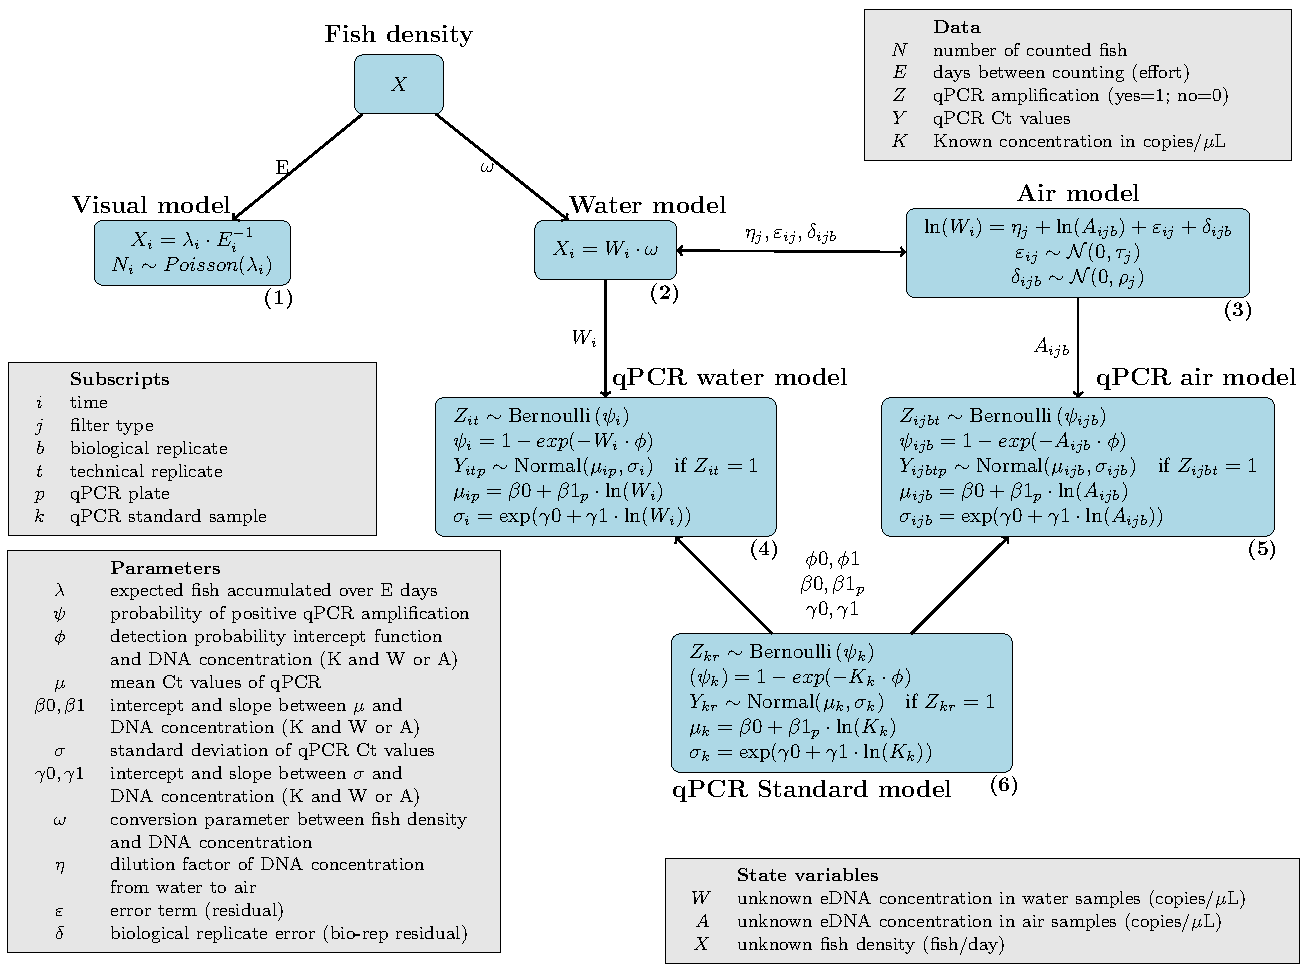
\includegraphics[width=16.5cm]{Plots/DAG.pdf}  
\caption{DAG of joint Bayesian model for estimating the eDNA concentration of Air}
\label{fig:DAG}
\end{figure}

\begin{table}[h]
    \centering
    \begin{tabular}{lll}
         & \textbf{Description} & \textbf{Prior} \\
&Data & \\
\hline
$N$ & number of fish counted & - \\
$E$ & elapsed days between counting & - \\
$Z$ & qPCR amplification (yes=1; no=0) & - \\
$Y$ & qPCR cycle threshold (Ct) & - \\
$K$ & known DNA concentration (qPCR standards) & - \\

&&\\
&State processes&\\
\hline
$X$ & unknown fish density in (fish $\cdot$ day$^{-1}$) & $\Gamma(10,1)$ \\
$W$ & unknown DNA concentration in water in (copies/$\mu$L) & - \\
$A$ & unknown DNA concentration in air in (copies/$\mu$L) & - \\
&&\\

&Transformed parameters&\\
\hline
$\lambda$& expected fish accumulated over E days & - \\
$\psi$& probability of positive qPCR amplification & - \\
$\mu$& mean Ct values of qPCR & - \\
$\sigma$& standard deviation of qPCR Ct values & - \\
&&\\

&Parameters&\\
\hline
$\omega$& conversion parameter between fish density
and DNA concentration & $\mathcal{N}(0,1)$\\
$\eta$& dilution factor of DNA concentration
from water to air & $\mathcal{N}(0,5)$\\
$\varepsilon$& time ($i$) specific error term (residual) & $\mathcal{N}(0,\tau)$\\
$\tau$& standard deviation of residuals & $\mathcal{TN}(0,1;0, +\infty)$\\
$\delta$& biological replicate error term (residual) & $\mathcal{N}(0,\rho)$\\
$\rho$& standard deviation of biological replicate error & $\mathcal{TN}(0,1;0, +\infty)$\\
$\phi$& intercept of the qPCR probability of detection ($\psi$) relationship &$\mathcal{N}(-1,1)$\\
& and eDNA concentration ($K$, $W$, and $A$) \\
$\beta0$& intercept of the linear relation between the mean Ct values ($\mu$)&$\mathcal{N}(40,1)$\\
&and eDNA concentration ($K$, $W$, and $A$) & \\
$\beta1$& slope of the linear relation between the mean Ct values ($\mu$) and &$\mathcal{N}(-3,1)$\\
&eDNA concentration ($K$, $W$, and $A$)) & \\
$\gamma0$& intercept of the linear relation between the standard deviation&$\mathcal{N}(1,0.1)$\\
&of Ct values ($\sigma$) and eDNA concentration ($K$, $W$, and $A$) & \\
$\gamma1$& intercept of the linear relation between the standard deviation &$\mathcal{N}(0,0.1)$\\
&of Ct values ($\sigma$) and eDNA concentration ($K$, $W$, and $A$) & \\
&&\\
&Index&\\
\hline
$i$& time (days) & -\\
$j$& filter type & -\\
$b$& biological sample replicate & -\\
$p$& qPCR plate & -\\
$k$& qPCR standard sample & -\\


    \end{tabular}
    \caption{Data, state processes, parameters, transformed parameters, and subscripts employed in the joint Bayesian model and their prior distributions}
    \label{tab:priortable}
\end{table}

\clearpage
\section{Results}
Here we present findings from connecting multiple observation methods (from traditional to contemporary to novel) for quantifying the abundance of coho salmon migration, including visual counting, river water eDNA sampling, and air-based eDNA passive filtration from aerosolized particles.

\subsection{Fish accumulation based on visual counts and eDNA in river water}
At first glance, time series data revealed that coho salmon migration occurs not as a single continuous event, but rather as a series of distinct burst peaks from mid-October through late November, where the peaks are highly likely to be connected with environmental factors such as water temperature and discharge. The average daily accumulation rate (X; black line in Figure \ref{fig:fig1}) was estimated at 133.7 fish/day with peaks exceeding up to 289 fish/day and low activity of ca. 35 fish/day (Figure \ref{fig:fig1}).

%Both observation methods (river water and visual observation) are a draw from the daily accumulation rate (X), the concordance between the two abundances was revealed on the robustness of the parameter $\omega$ = 7.35 (6.99 and 7.73 lower and upper 95\% quantile) indicating that the accumulation of 1 fish/day would equal $\approx 1500$ ($\pm 500$) copies/$\mu$L reaction.

Because both observation methods (river water eDNA and visual observation) are jointly used to estimate the daily accumulation rate (X), their concordance was best evaluated through the parameter $\omega$. A converged and narrowly distributed $\omega$ parameter indicates strong agreement between the two methods and simultaneously a reliable conversion parameter from fish/day to eDNA copies/$\mu$L. In this case, $\omega$ = 7.35 (95\% quantile range of 6.99 to 7.73), suggesting consistent concordance between observed fish counts and eDNA concentrations hence, biologically, this implies that an accumulation rate of 1 fish/day corresponds to approximately 1500 ($\pm$ 500) copies/$\mu$L per reaction.

\begin{figure}[tbhp] 
\centering
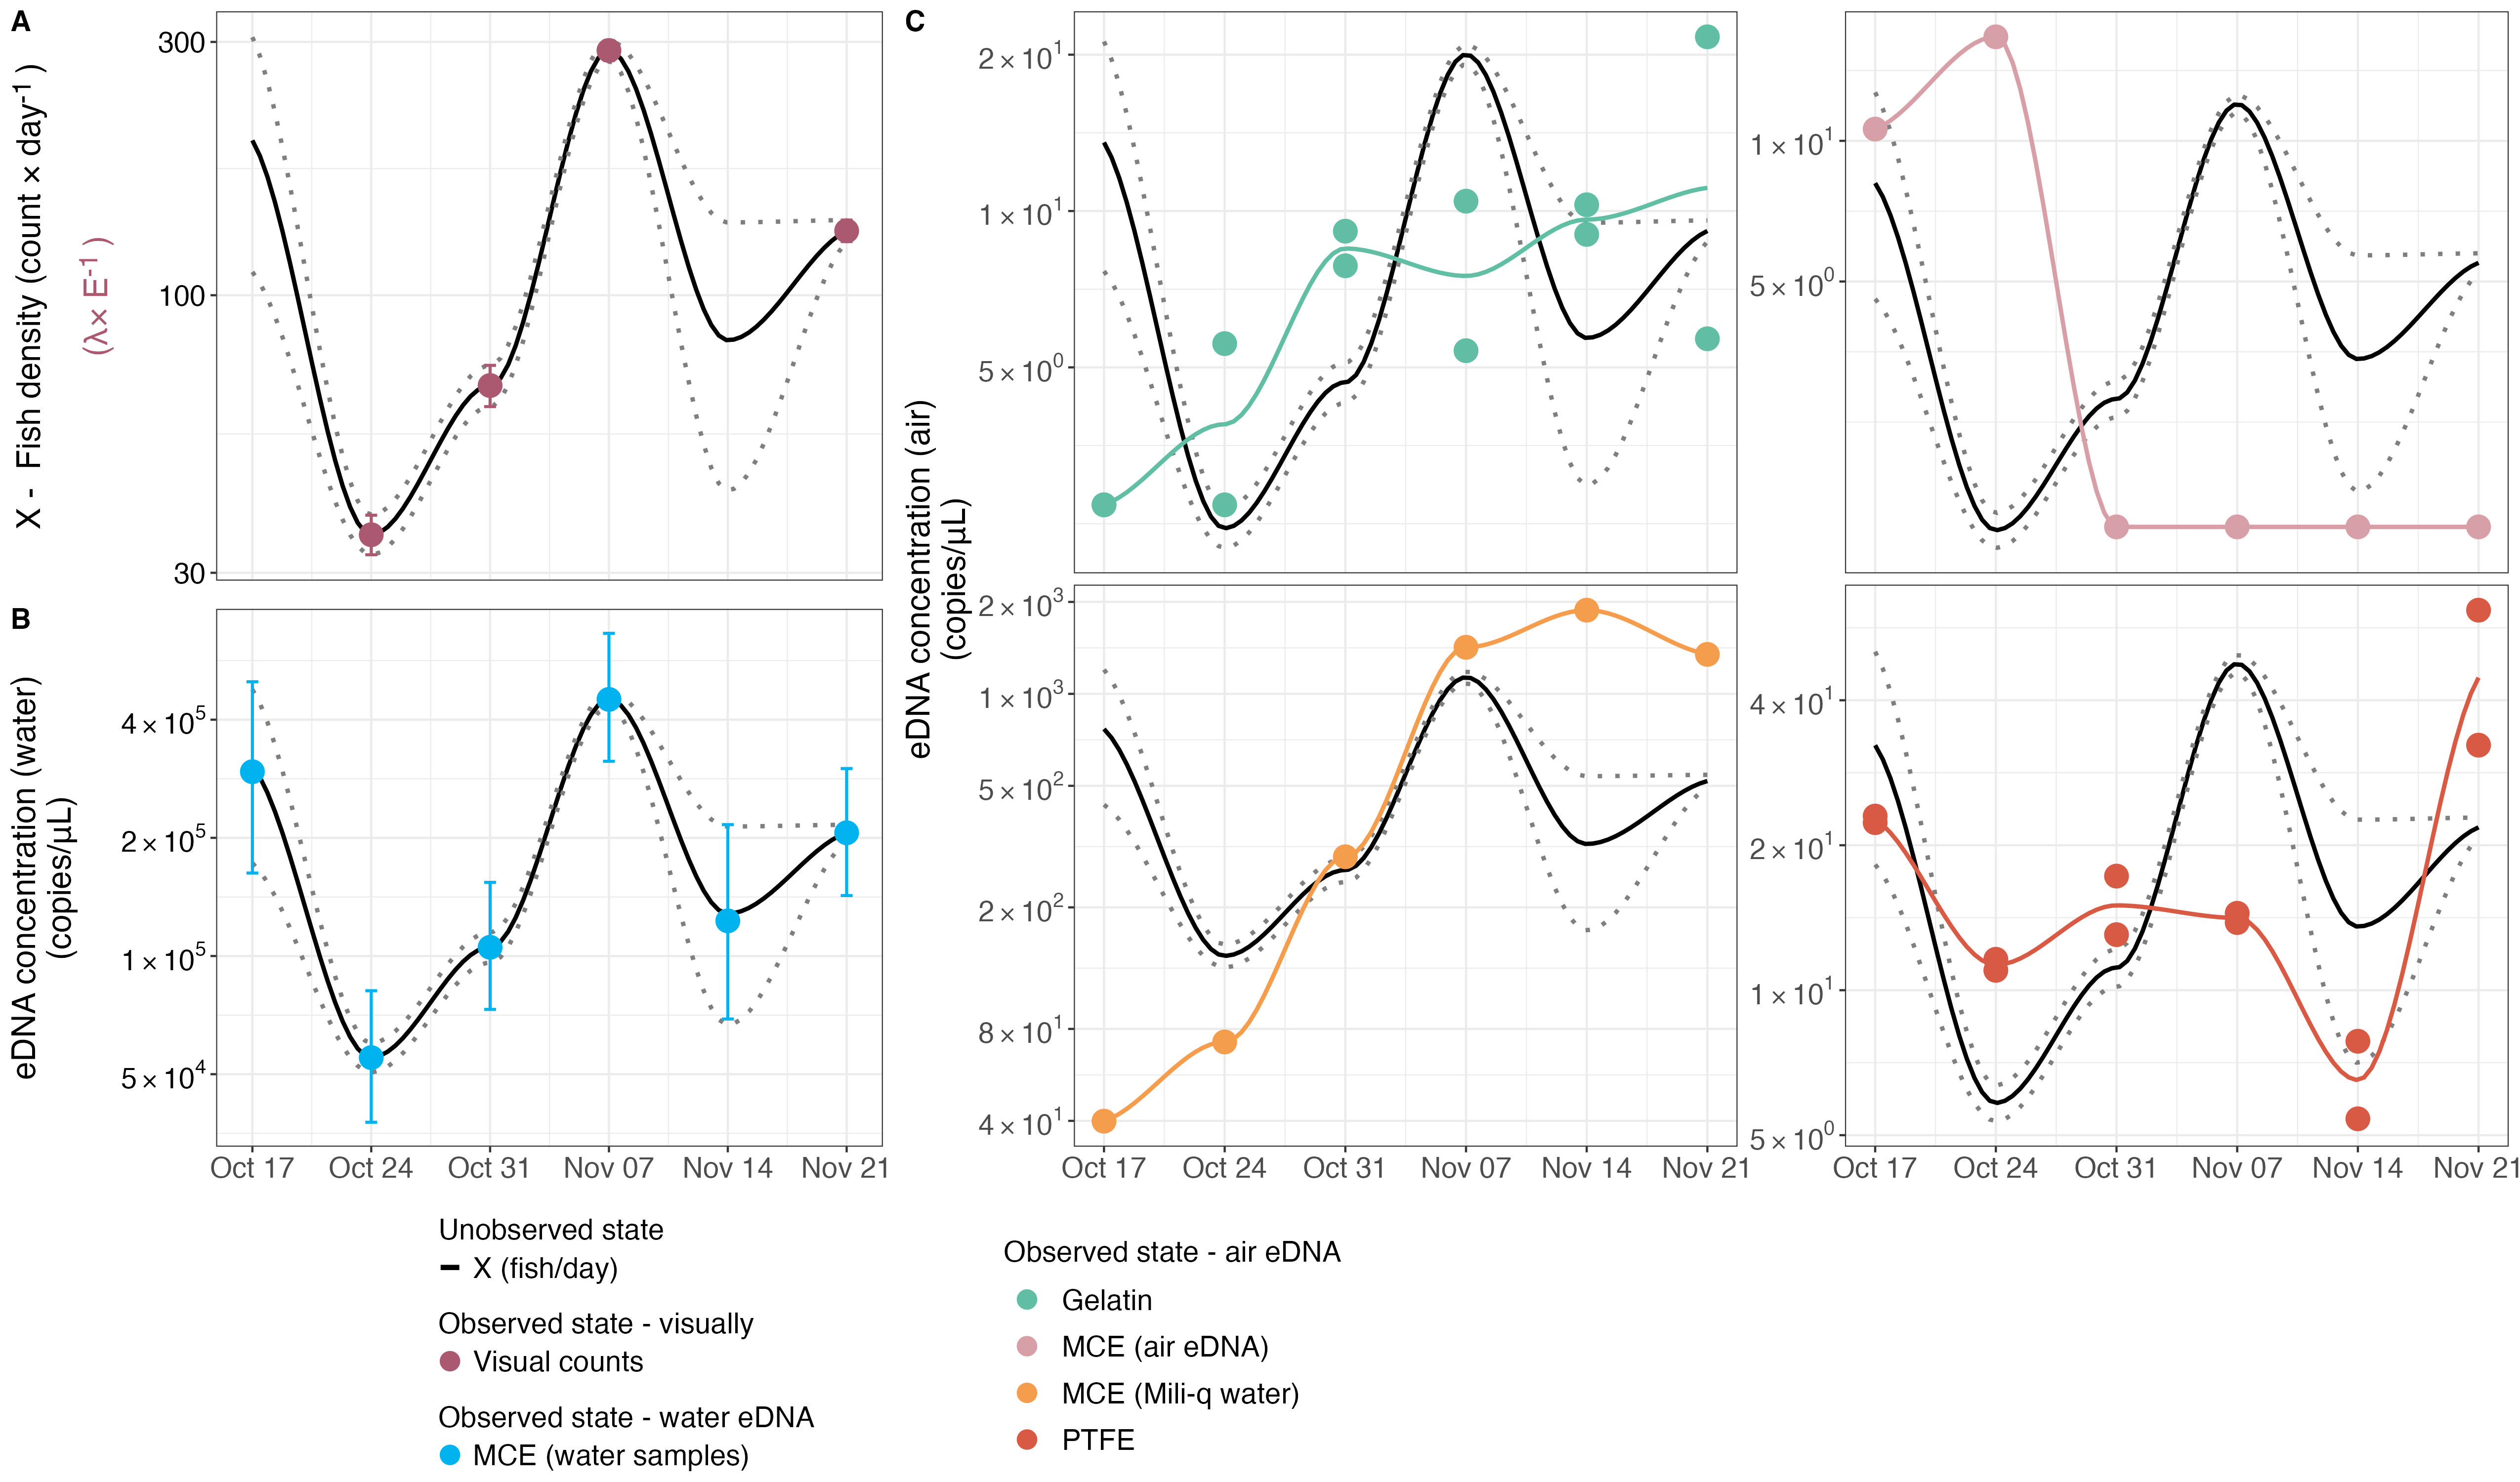
\includegraphics[width=16.5cm]{Plots/Figure_1.jpg}  
\caption{The temporal dynamics of estimated fish density (X; black line with 95 confidence intervals - dotted lines) from October 17$^{th}$ to November 21$^{st}$ compared to the posterior distributions of visual observations (A), eDNA concentrations in water (B), and eDNA concentrations in water using various filter types (C).}
\label{fig:fig1}
\end{figure}


\subsection{Air eDNA signals}
Airborne eDNA originating from coho salmon was successfully detected across all passive air collection methods deployed (gelatin, PTFE, MCE filters suspended in air, and open containers of deionized water - MCE DI water). These results provide compelling proof-of-concept evidence that genetic material from aquatic organisms can be recovered from the atmosphere without requiring active airflow systems, thereby demonstrating the viability of fully passive sampling approaches for detecting airborne aquatic eDNA under field conditions.

Although all air sampling methods successfully detected the presence of upstream migratory coho salmon, we observed significant differences in recovery efficiency among filter types (Table \ref{tab:filter_error}). The airborne environmental was recovered at varying quantities through different collection methods, with the highest recovery observed in the open containers filled with deionized water (MCE DI water), where eDNA concentrations were approximately 5.3-fold diluted compared to those measured directly in river water samples.
In contrast, suspended filter exhibited substantially lower eDNA concentrations, hence higher dilution factors: PTFE showed approximately 8.4-fold dilution, gelatin showed 9.3-fold dilution, and MCE air demonstrated the highest dilution at 9.8-fold. These differences in dilution factors reflect the varying capacities and efficiencies of different collection methods in capturing and retaining airborne aquatic eDNA from the environment.

In terms of alignment with the biological activity, PTFE and gelatin filters best mirrored the daily fish accumulation patterns, exhibiting the lowest residual errors ($\varepsilon$ = 0.570 and 0.788, respectively).  Conversely, MCE DI water, despite recovering the highest eDNA concentration, showed less parsimony with the fish migration dynamics ($\varepsilon$ = 0.974; Figure \ref{fig:fig1}). The MCE air suspended filters performed least effectively in tracking temporal migration patterns, failing to amplify coho salmon DNA beyond the first two weeks of the sampling campaign.

Subsequently, biological replicates for gelatin and PTFE filters revealed additional insights regarding methodological robustness and reproducibility. PTFE filters produced the most consistent quantifications, with lower variance between replicates ($\delta$ = 0.106), whereas gelatin filters showed a higher degree of variability ($\delta$ = 0.230), indicating reduced reproducibility of quantitative outcomes. 

These findings underscore the importance of filter selection in both the sensitivity and reliability of airborne eDNA monitoring.

\begin{table}[h!]
\centering
\caption{Error measurements for different filter types}
\label{tab:filter_error}

\begin{tabular}{llll}
\textbf{Filter type} & \textbf{Dilution ($\eta$)} & \textbf{Error ($\overline{|\varepsilon|}$)} & \textbf{Biological rep error ($\overline{|\delta|}$)} \\
Gelatin & $e^{-9.25}$ & 0.788 & 0.230 \\
PTFE & $e^{-8.39}$ & 0.570 & 0.106 \\
MCE Air & $e^{-9.77}$ & 1.370 & - \\
MCE DI water & $e^{-5.33}$ & 0.974 & - \\
\end{tabular}
\end{table}


\subsection{Model diagnostics}

Convergence and reliability of the Bayesian model were assessed through comprehensive diagnostics. All parameters (Table \ref{tab:priortable}) exhibited Gelman-Rubin convergence statistics ($\hat{R} < 1.01$) and effective
sample sizes (ESS) exceeding 1000 per parameter, indicating successful convergence and efficient mixing of
the six independent chains (Figure \ref{fig:diagnostics}\textit{A}). 


No divergent transitions were detected during sampling, and the maximum tree depth was not exceeded, indicating no issues with divergence or exploration limits (Figure \ref{fig:diagnostics}\textit{B}). The posterior likelihood demonstrated convergence before the sampling phase began, with all chains exhibiting high mixing, confirming robust exploration of the parameter space (Figure \ref{fig:diagnostics}\textit{B}).

Prior sensitivity analyses revealed that posterior estimates differed from priors, demonstrating that the posteriors were appropriately updated based on the observed data rather than being heavily influenced by prior assumptions (Figure \ref{fig:prior_sens}). Additionally, the posterior predictive checks (PPC) demonstrated that the model reliably reproduced the observed data, supporting the validity of parameter estimates (Figure\ref{fig:prior_sens}). 

Collectively, these diagnostics confirm the reliability and validity of the Bayesian model used here.

\begin{figure}[tbhp] 
\centering
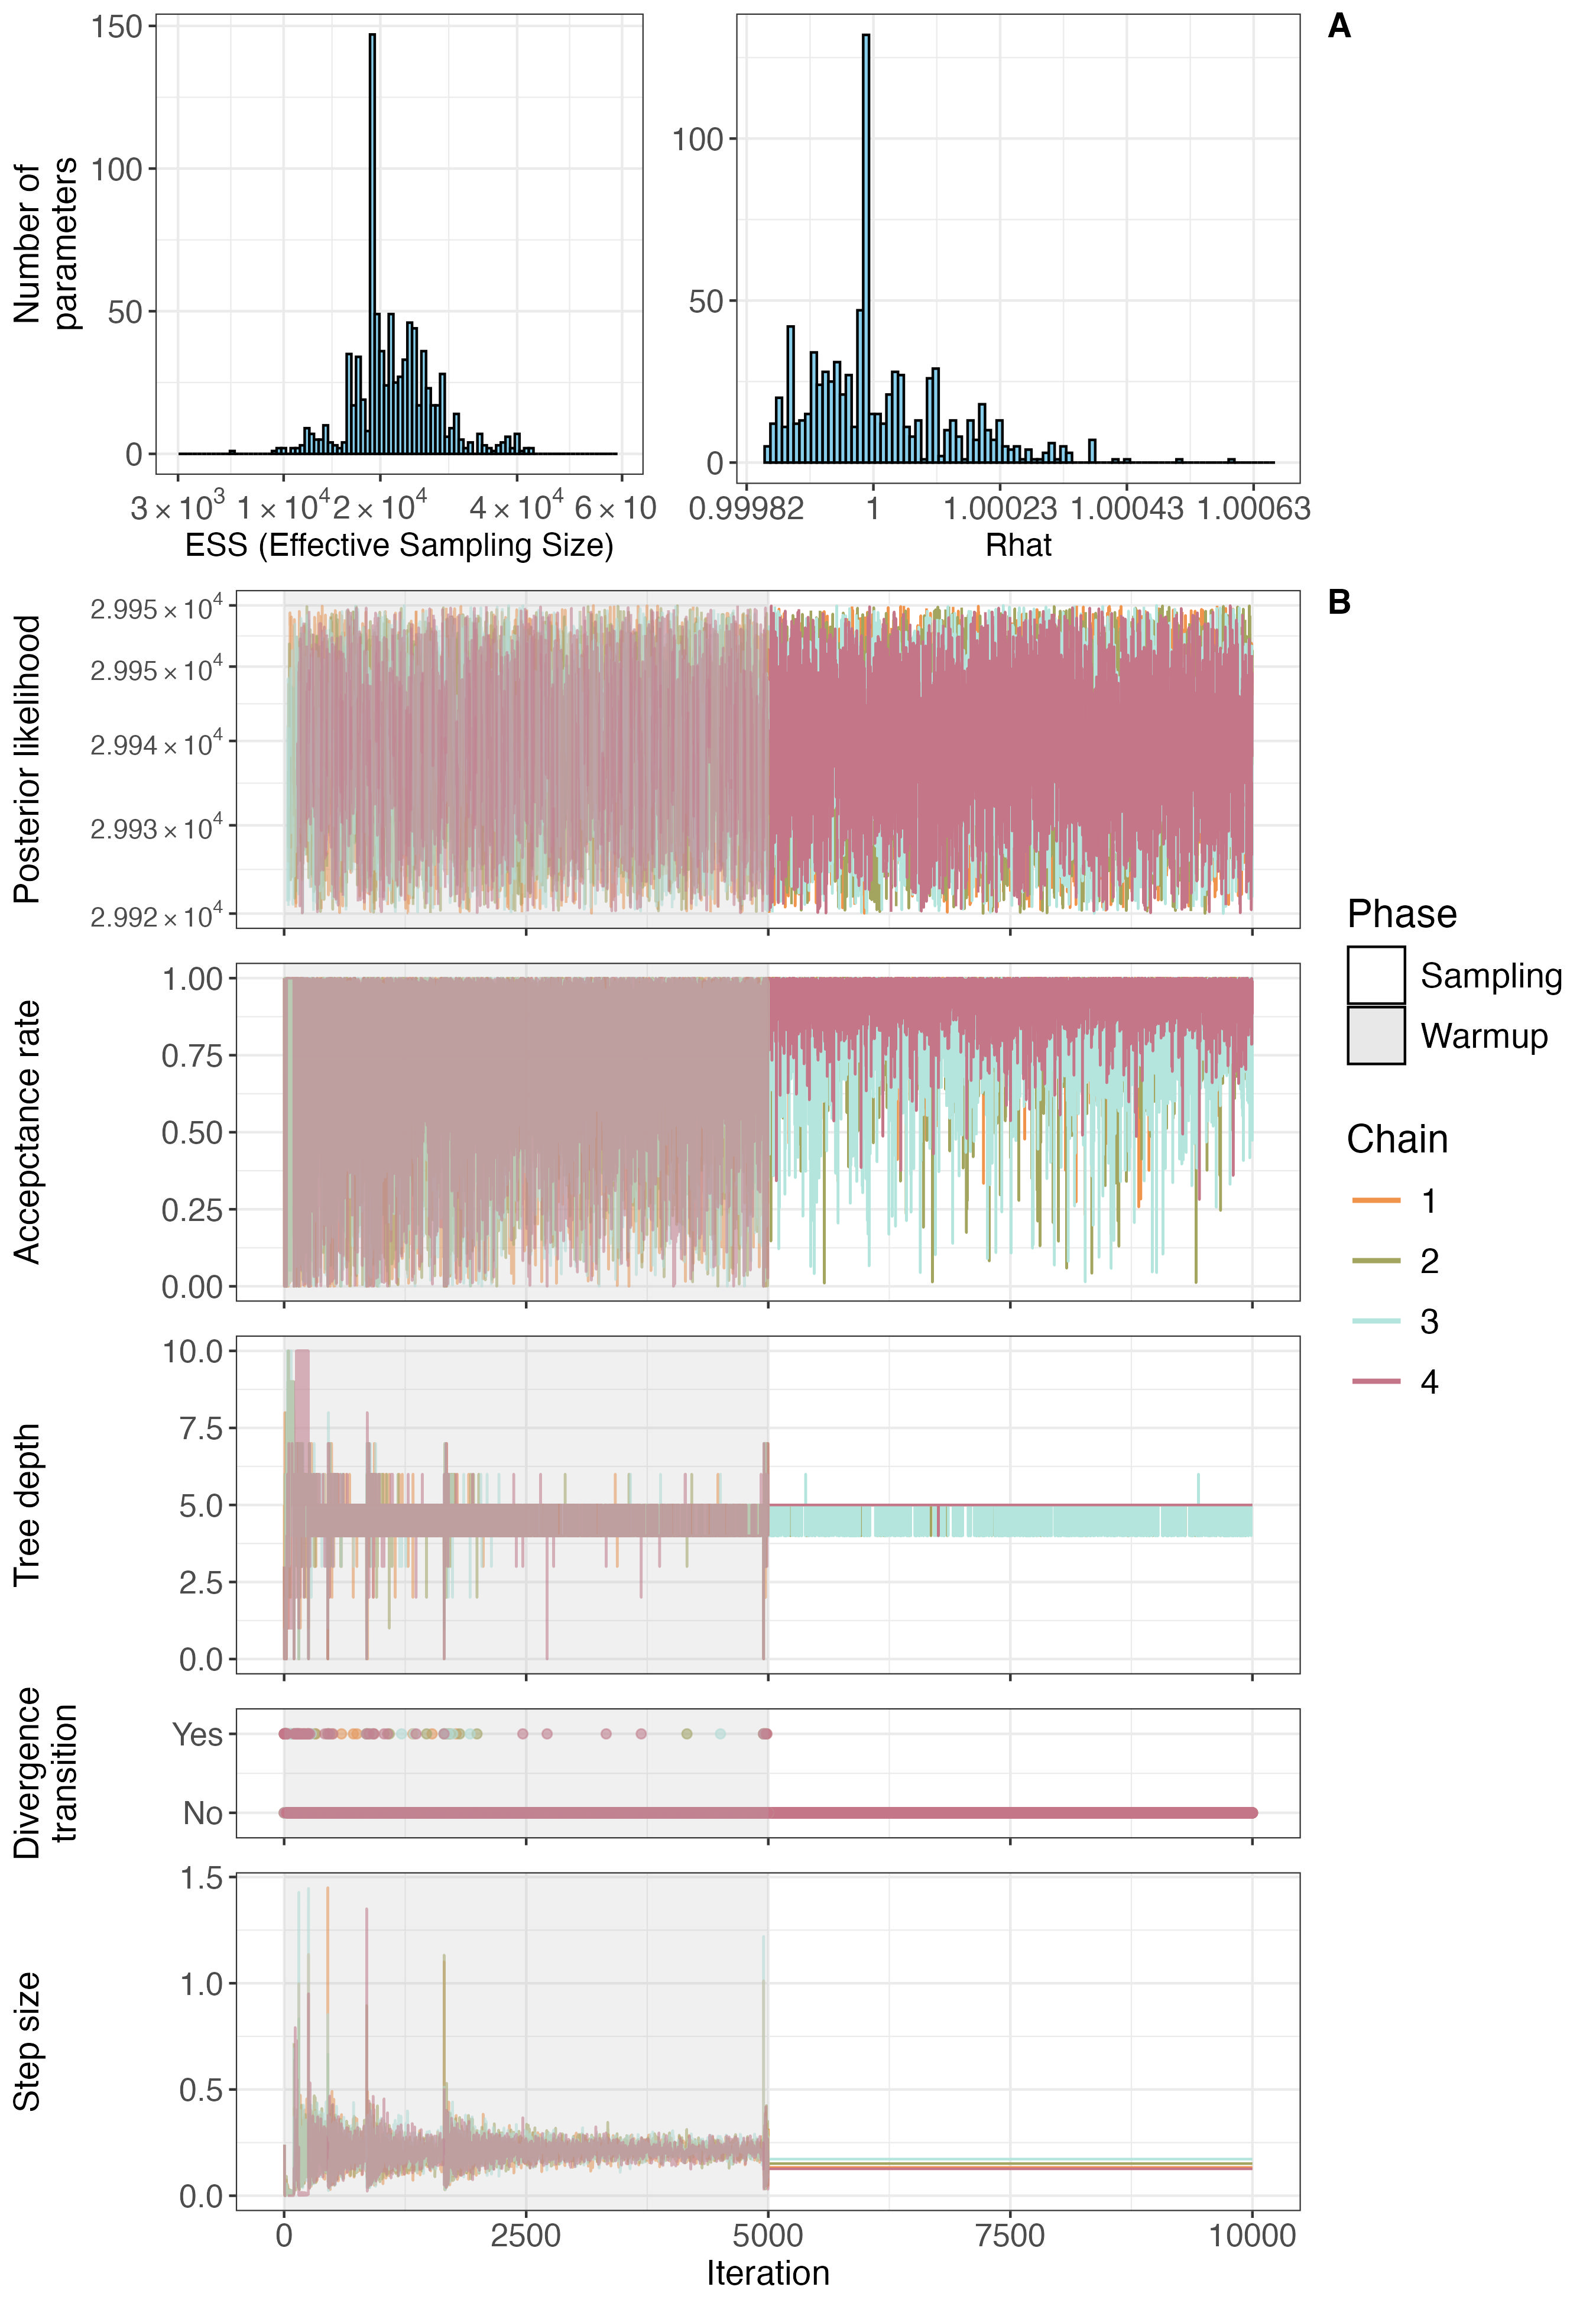
\includegraphics[width=16.5cm]{Plots/Diagnostic_Fig_1.jpg}  
\caption{Model diagnostics}
\label{fig:diagnostics}
\end{figure}


\begin{figure}[tbhp] 
\centering
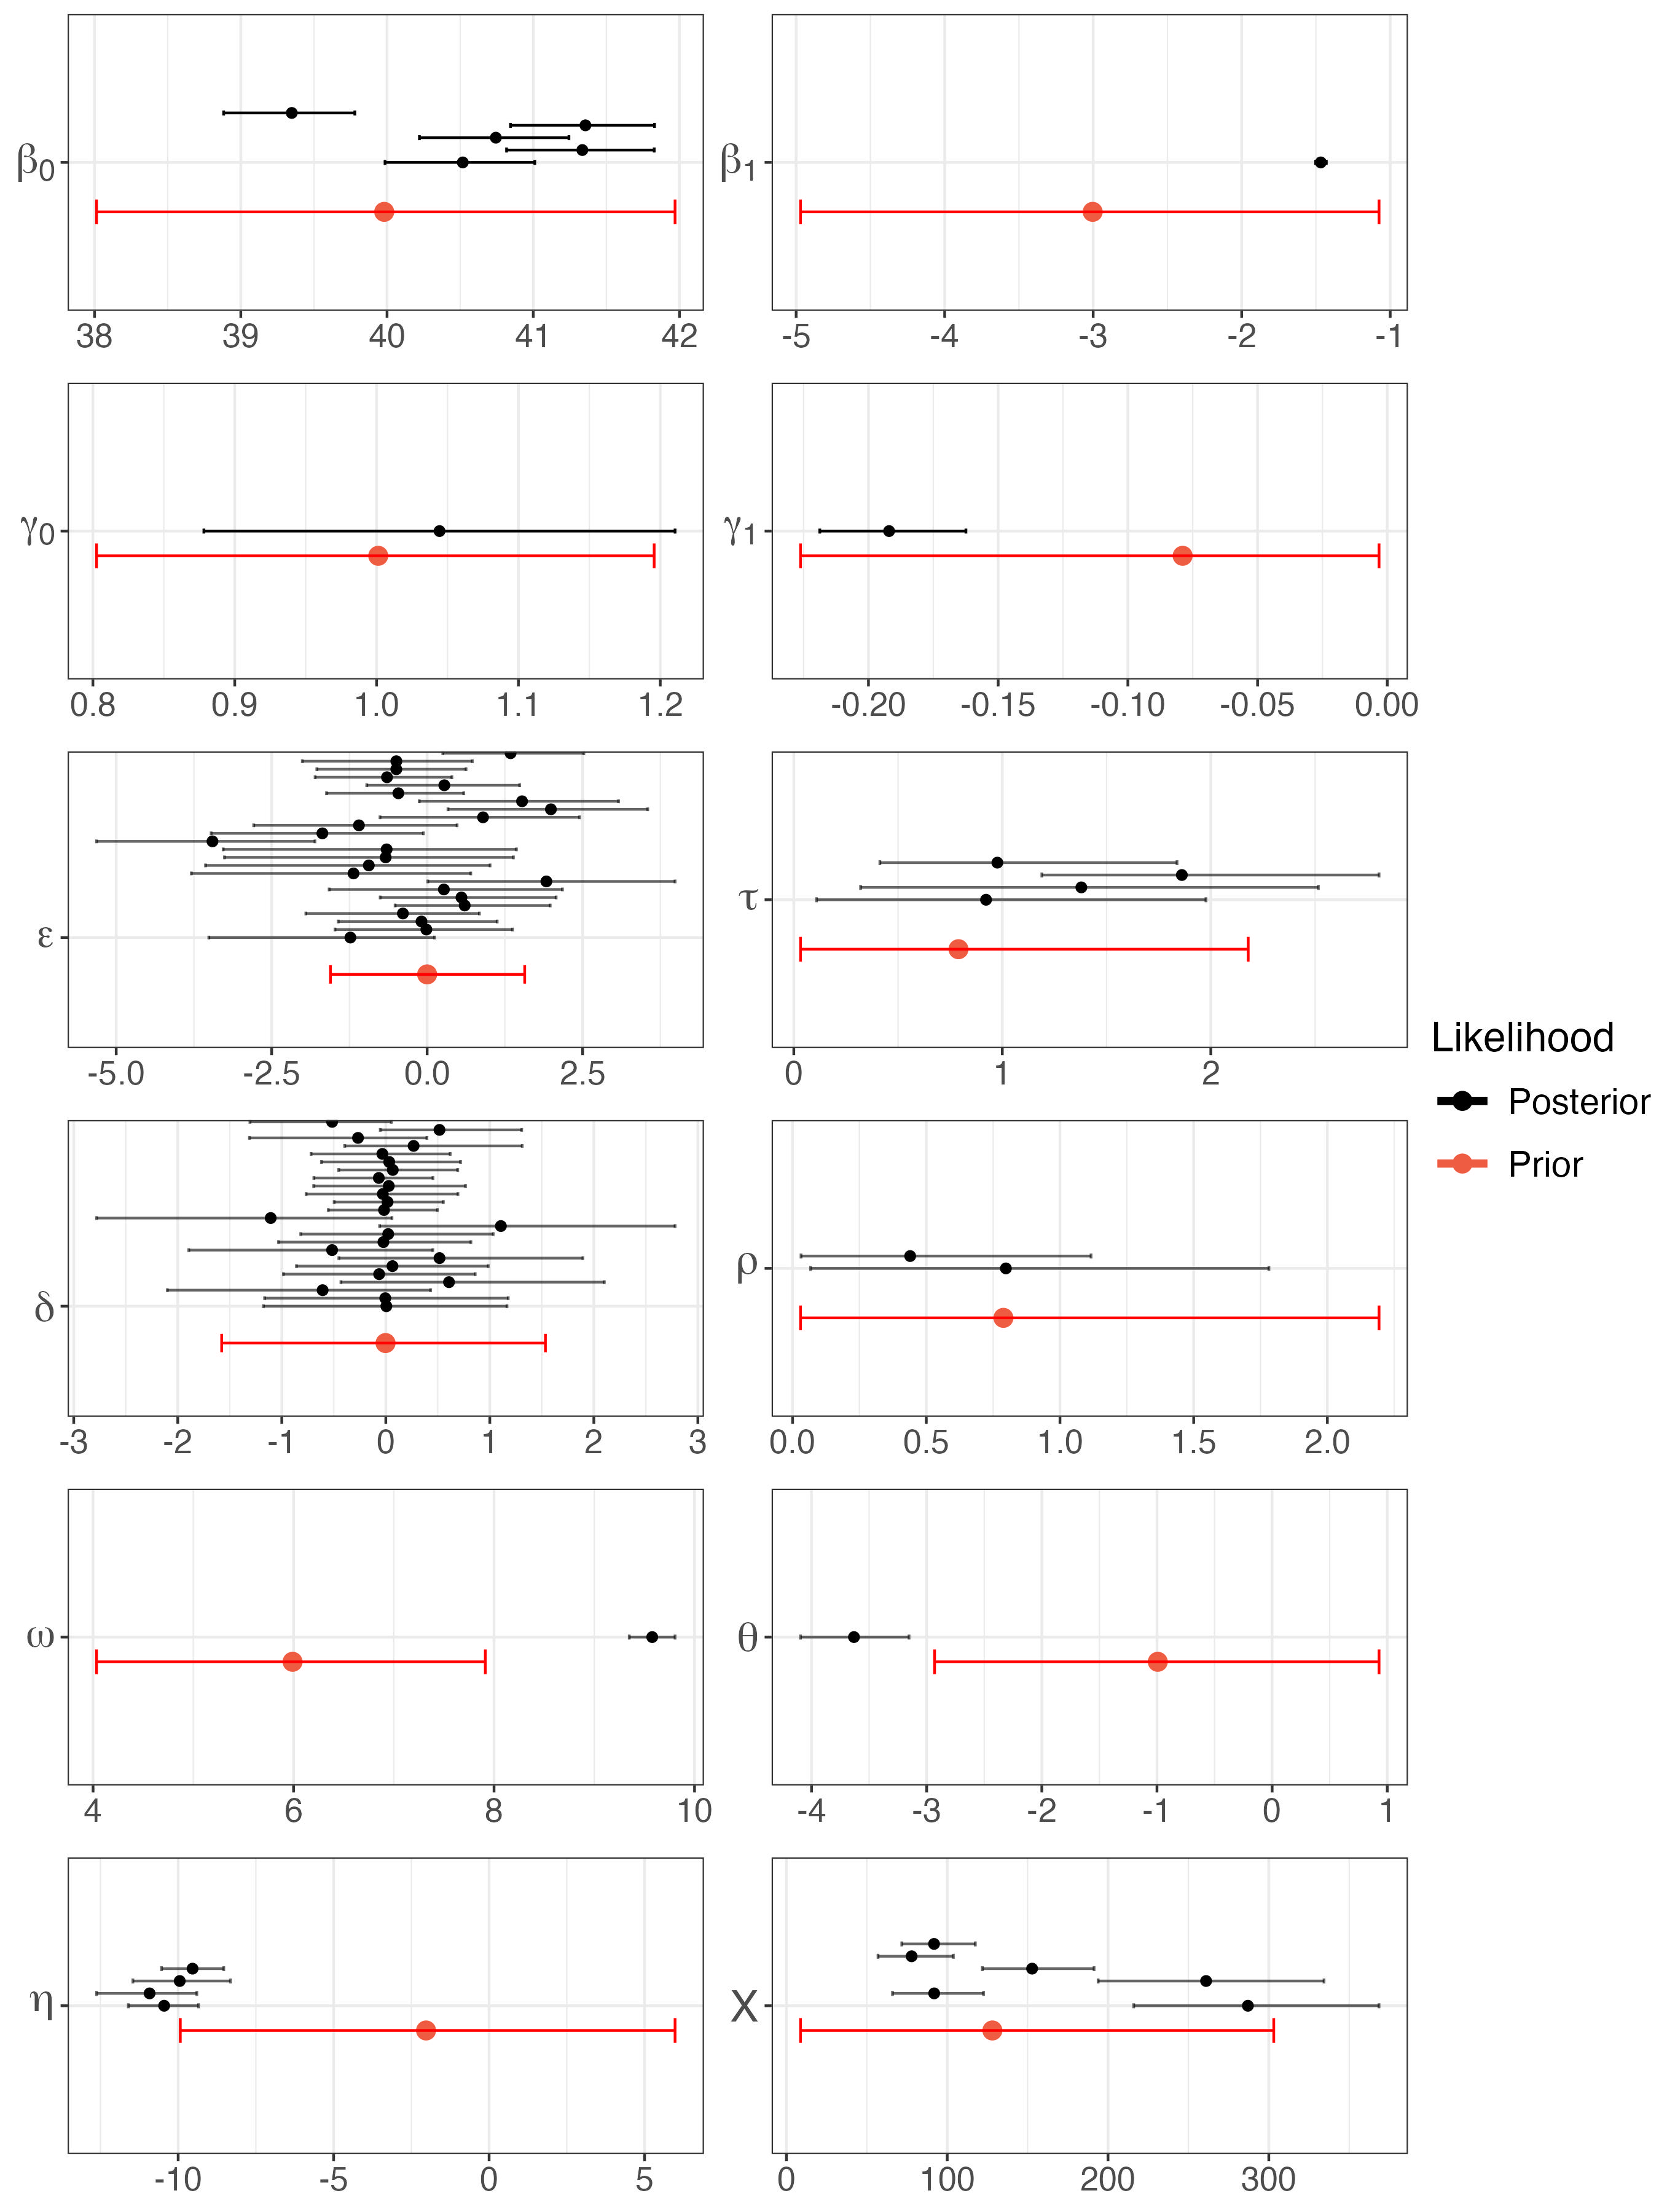
\includegraphics[width=16.5cm]{Plots/Diagnostic_Fig_2.jpg}  
\caption{Prior sensitivity analysis}
\label{fig:prior_sens}
\end{figure}

\section{Discussion}
Our study establishes, for the first time, that passive airborne environmental DNA (eDNA) sampling can reliably capture and quantify molecular signals from aquatic organisms. This represents a paradigm shift in how we access aquatic biodiversity—through the air, without ever touching the water. Results from salmon spawning streams demonstrate that DNA from aquatic habitats is transported into the atmosphere by natural processes such as evaporation, aerosolization, and splashing. Data obtained from multiple passive collection methods, validated against conventional water-based eDNA assays and direct visual counts, reveal a robust quantitative link between airborne DNA concentrations and observed salmon density. Although airborne eDNA signals are typically low, our sensitive methodologies and advanced statistical models enabled the detection of clear quantitative patterns. These findings not only confirm the presence of aquatic eDNA in the air—it opens an entirely new front in ecological monitoring, providing compelling evidence that these signals serve as a quantitative proxy for monitoring population abundance. In doing so, they challenge the traditional view that aquatic biological signals are confined solely to water and underscore the deep interconnectedness of environmental systems (REF). By extending the reach of aquatic biomonitoring into the air, this work heralds a transformative shift in our ability to surveil biodiversity in a non-invasive and scalable manner, particularly as ecosystems grow more dynamic and less accessible due to climate change.

The insights regarding the atmosphere as a sampling medium are particularly noteworthy. Our observations support the ‘air is dilute water’ hypothesis by demonstrating that DNA molecules shed by aquatic organisms are carried upward and remain detectable using passive sampling techniques, particularly when these airborne particles settle. Key transport mechanisms include evaporation, aerosol formation, and mechanical disturbances such as splashing and the leaping behavior of salmon. Environmental variables, including wind, humidity, and temperature, strongly influence the dispersion and concentration of airborne eDNA (REF). For example, under humid conditions, airborne particles tend to settle rapidly and rainfall washes them downward, resulting in highly localized deposition (REF). In our vertically deployed passive system with the open container of deionized water, gravitational settling appears to be the predominant mechanism of eDNA deposition. This vertical orientation takes advantage of the natural tendency of airborne particles to eventually fall, regardless of how they enter the air, whether through aerosolization, evaporation, or splashing. In contrast, filters deployed in a horizontal orientation, such as the hanging PTFE, gelatin, and MCE filters, require airborne particles to be laterally displaced by wind in order to make contact with the filter surface. Without active airflow, this setup is likely less efficient at capturing settling particles. Nonetheless, many prior airborne eDNA studies have employed horizontal filter orientations in conjunction with active air pumps. These powered systems draw large volumes of air across the filters, potentially compensating for orientation by forcefully transporting particles onto the collection surface. However, this advantage comes with a trade-off: the pumping action draws from a broader spatial catchment, likely reducing the ability to pinpoint local ecological variation (REF). Thus, the optimal configuration for airborne eDNA sampling, whether vertical or horizontal, passive or active, may ultimately depend on environmental conditions and the resolution goals of a given study. Moreover, because passive collection does not rely on pump-driven flow rates or collection medium volumetric measurements, quantification is based solely on the collector’s exposed surface area and deployment duration, which is a non-standard metric that complicates direct comparisons with conventional methods. Despite this limitation, the reliance on natural gravitational settling may enhance localized resolution, providing critical insights into microhabitat variations and subtle ecological dynamics (REF).

Filter material and deployment considerations are also critical to the performance of airborne eDNA sampling. In our study, passive collection devices containing filters made from gelatin, PTFE, and MCE, along with an open container of deionized water, were deployed under field conditions. Our results indicate that PTFE filters, which offer high material durability, delivered the greatest reproducibility across replicates, while gelatin filters yielded the highest sensitivity, albeit with increased environmental variability. In contrast, MCE filters performed very poorly, which is unsurprising given that they are primarily designed for water filtration rather than airborne sampling. Notably, the open deionized water container, offering a surface area of approximately 750 cm² compared to roughly 16 cm² for the small circular filter disks (~47 mm in diameter), achieved the highest overall DNA recovery. An additional factor to consider is the operational context. In heavy rainfall, for example, the open container method may capture more DNA simply due to larger surface area and additional water input, but it fundamentally still requires a pump to process and filter the collected water, adding logistical complexity. In contrast, PTFE filters, which work well under wet conditions, do not require such equipment. Similarly, while gelatin filters yield higher DNA amounts, they are best suited for dry conditions due to their increased environmental sensitivity. Additionally, the optimal deployment duration for passive airborne eDNA remains relatively unknown. Longer exposures may accumulate more settled material, but risk increased degradation due to environmental factors such as exposure to UV radiation, microbial activity, or moisture. Identifying this balance will be critical to maximize signal recovery while preserving DNA integrity. Collectively, these factors represent important knowledge gaps that future studies should address through systematic investigations of filter design, orientation (vertical versus horizontal), and exposure duration (REF).

Perhaps most striking is the simplicity and versatility of this approach. With no need for pumps, power, or complex infrastructure, passive airborne eDNA sampling enables the recovery of deep biological signals through minimal sampling effort. Beyond its elegance, the method offers substantial practical advantages: it is non-invasive, scalable, and significantly reduces operational risks compared with traditional water sampling, particularly in remote or hazardous environments where logistical constraints are severe. By integrating multiple data streams from visual surveys, water-based eDNA analyses, and airborne eDNA measurements, the current study demonstrates enhanced estimation accuracy of aquatic populations. Moreover, the capacity to capture quantitative data from the air offers significant potential for real-time monitoring of dynamic ecological processes. Nevertheless, challenges remain. Detections at very low DNA concentrations remain problematic, and the performance of passive filters can fluctuate with changes in weather, ambient temperature, and other environmental conditions. Additionally, our current sampling design, which relied on overnight 24-hour deployments, provides limited temporal resolution. These limitations underscore the need for further methodological refinements, including the development of continuous or automated sampling systems and the integration of advanced statistical models that account for environmental variability (REF).

The broader implications of this work extend beyond technical validation. This study not only validates a new method—it reimagines what is possible in environmental surveillance. This novel capability is not limited to pristine or remote systems; it holds equally transformative potential for urban wetlands, stormwater channels, and even cities, where direct water sampling may be logistically challenging or hazardous. By demonstrating that ecological signals from aquatic systems can be effectively captured in the air, this study challenges conventional assumptions about the spatial boundaries of ecological and biological monitoring. Expanding the sampling domain into the atmosphere offers a powerful new tool for high-resolution, real-time biodiversity surveillance that is both cost-efficient and scalable across extensive geographic areas. This innovative approach holds significant promise for environmental genomics, conservation biology, and fisheries management. For example, remote or hazard-prone regions that have previously been difficult to monitor could now be continuously surveyed, thereby improving early warning systems for population declines, invasive species incursions, or pathogen outbreaks. Furthermore, the potential to detect pathogens such as Escherichia coli or Legionella pneumophila directly from airborne samples opens new avenues for public health monitoring in environments where water sampling poses risks (REF). The integration of drone-based deployment and retrieval of passive air samplers is also a promising avenue for dramatically upscaling this technique, enabling extensive automated monitoring without the logistical constraints associated with traditional methods (REF; Geckeler 2025; Kirchgeorg et al., 2024).

Future research should focus on enhancing sensor design and further optimizing passive collection techniques. Key areas for investigation include systematic studies on filter orientation, size, and deployment duration, as well as controlled experiments evaluating the effects of meteorological factors such as wind, humidity, and temperature on eDNA deposition. Expanding research to encompass a broader array of aquatic species and ecosystems, along with longitudinal studies to capture seasonal variations and responses to environmental stressors, will be essential for refining quantitative models. Additionally, the development and standardization of protocols for the collection and analysis of airborne eDNA will be crucial for ensuring reproducibility and comparability across studies and regions. Ultimately, the findings presented herein lay a transformative foundation for ecological monitoring by integrating insights from both aquatic and atmospheric sciences, and they offer a new paradigm for the real-time, comprehensive management of natural resources in a rapidly changing environment (REF).

\section*{Acknowledgments}
We thank Natasha Kacoroski, Larry Franks, and the dedicated volunteers at Friends of the Issaquah Salmon Hatchery for their generous support in the field. We are also grateful to Travis A. Burnett and Darin Combs at the Washington Department of Fish and Wildlife for facilitating access and permitting field experimental work at the Issaquah Hatchery. Additional thanks to Pedro F.P. Brandão-Dias for assistance with air filter deployments, and to Kevan Yamanaka at the Monterey Bay Aquarium Research Institute for designing and fabricating the 3D-printed passive filter holders. We are especially grateful to Chris Sergeant for valuable insights on salmon biology that shaped the interpretation of our findings. We acknowledge funding support from OceanKind [Grant No. GR042390] and the Packard Foundation [Grant No. GR016745] and thank the Centre of Environmental Genomics for providing access to high-performance computing resources.

\section*{Author contributions}
Y.C.A.I. conceived the study. Y.C.A.I. G.G and E.A.A. designed the field and laboratory protocols. Y.C.A.I. and G.G. jointly designed the downstream statistical analyses and Bayesian modeling framework. G.G. conducted all statistical analyses, with inputs from R.P.K. The fieldwork was performed by Y.C.A.I. and E.A.A., while Y.C.A.I. and G.G. co-wrote the manuscript. R.P.K. supervised the project, contributed to conceptual guidance, and provided critical revisions. All authors contributed to the study design and approved the final manuscript.  

\section*{Data availability}
The authors declare that they have no competing interests. All data needed to evaluate the conclusions in this paper are available in the main text and/or the Supplementary Materials. Additional data, code, and materials will be made available upon reasonable request. No materials were subject to material transfer agreements (MTAs).

\clearpage
\bibliography{Bib.bib}
\end{document}


\begin{table}[h]
    \centering
    \begin{tabular}{llll}
        \textbf{Filter type} & \textbf{Dilution ($\eta$)} & \textbf{Error ($\overline\varepsilon$)} & \textbf{Biological rep error ($\overline\delta$)} \\
        Gelatin & $e^{-9.5}$ & 0.628 & 1.315 \\
        PTFE & $e^{-8.8}$ & 0.666 & 0.682 \\
        MCE air filter & $e^{-10.2}$ & 1.133 & - \\
        DI water & $e^{-5.7}$ & 0.606 & - \\
    \end{tabular}
    \caption{Error measurements for different filter types}
    \label{tab:filter_error}
\end{table}



Fish Density Model (Water): The number of fish counted ('N') at a given point is assumed to be proportional to the total amount of water-borne DNA, which can be estimated from measurements taken underwater and converted into an 'eDNA concentration' parameter ('W'). This conversion process involves multiplying by another factor called 'omega', denoted as 'ω'.
Air Model: The eDNA concentrations in air samples are calculated based on those found in the corresponding water sample using a dilution factor, which is determined from measurements taken underwater and above ground (i.e., atmospheric pressure). These factors include both known ('K') and unknown values of DNA concentration that need to be estimated during model fitting or inference processes.
qPCR Model: The number of positive amplification results in the various types of samples are assumed to follow a Poisson distribution, with mean proportional to their respective eDNA concentrations (W for water-borne species) as well as effort ('E', which represents days between counting). This relationship is captured by parameters like 'phi0' and 'phi1'.
Visual Model: The probability of finding fish in an underwater visual census survey follows a logistic model, with the logit link being determined by linear combinations involving eDNA concentration (W) as well as other covariates ('X') such as depth or temperature measurements taken at each counting event. This relationship is represented by parameters like 'beta0' and 'beta1'.
Standard Model: In cases where a known standard sample with DNA content of K copies/μL exists, the model allows for estimation of eDNA concentrations in water samples ('W') using this reference value as well as other covariates (X). The relationship is determined by parameters like 'gamma0' and 'gamma1'.
Error Terms: Various error terms are included to account for uncertainty or variability introduced during different stages of the analysis process, such as biological replicates in air sampling ('delta b'), residuals from model equations involving eDNA concentration (omega), dilution factors between water-borne vs atmospheric DNA samples (eta) and technical replicate measurements taken within each type of sample. By incorporating these relationships into a single graphical structure that can be analyzed using statistical software, researchers are able to estimate parameters like 'W', 'A' or other key ecological variables with improved accuracy compared to traditional methods relying solely on one specific analytical technique alone (e.g., qPCR).

We can start by defining λ as fish density, where ω represents a conversion parameter from fish/day to copies/μL (the unit for DNA concentrations). This means that W = λ * ω and $A_b = η^(-1)$ / B. The air model also includes the δ error term representing biological replicate differences between samples taken at different times or using different filters, leading to a final equation of:
Aij= (ηj + ln(PB))/B with PB being an unknown constant that depends on both filter type and bioreplicate difference in time. The qPCR water model can be defined similarly as $Z = ψ_i * W^(-1)$ where μ is the mean Ct values of a standard curve, β represents slopes between DNA concentration (K or A), σ being its corresponding error term for each sample i at different times t during counting and plate p. The qPCR air model can be defined as $Z = ψ_k * K^(-1)$ with μ representing the mean Ct values of a standard curve, β represents slopes between DNA concentration (K or A), σ being its corresponding error term for each sample i at different times t during counting and plate p. The qPCR Standard model can be defined as $Z = ψ_i * W^(-1)$ with φ representing intercepts/slopes of the probability response to standard curve concentrations K, μ mean Ct values from a single amplification cycle (Ct), σ being its corresponding error term for each sample i at different times t during counting and plate p. The parameters can be estimated using maximum likelihood estimation or Bayesian methods such as MCMC sampling if needed given prior distributions specified on all unknown quantities including $W_i = η^(-1) / B$ with PB representing an unknown constant that depends both filter type bioreplicate difference in time, ε error term (residual), and δ being biological replicate errors. The subscripts provide information about the variables at different times i during counting or using filters jb for each sample b taken over multiple plates pqPCR standard samples k
